\documentclass[12pt]{article}
\usepackage[usenames]{color} %used for font color
\usepackage{amssymb} %maths
\usepackage{amsmath} %maths
\usepackage{graphicx}

\newcommand{\GeV}{\ensuremath{\mathrm{GeV}}}
\newcommand{\TeV}{\ensuremath{\mathrm{TeV}}}
\newcommand{\GeVc}{\ensuremath{\mathrm{GeV}}}
\newcommand{\TeVc}{\ensuremath{\mathrm{TeV}}}
\newcommand{\GeVcc}{\ensuremath{\mathrm{GeV}}}
\newcommand{\TeVcc}{\ensuremath{\mathrm{TeV}}}
\newcommand{\pt}            {\ensuremath{p_{\mathrm{T}}}\xspace}
\newcommand{\kt}            {\ensuremath{k_{\mathrm{T}}}\xspace}
\newcommand{\antikt}        {anti-\kt}
\newcommand{\ttbar}        {\ensuremath{\mathrm{t}\overline{\mathrm{t}}}}
\newcommand{\bbbar}        {\ensuremath{\mathrm{b}\overline{\mathrm{b}}}}
\newcommand{\qqbar}        {\ensuremath{\mathrm{q}\overline{\mathrm{q}}}}
\newcommand{\fbinv}        {\ensuremath{\mathrm{fb}^{-1}}}
\newcommand{\instlumiA}     {\ensuremath{\times 10^{33} \mathrm{cm}^{-2} \mathrm{s}^{-1}}}
\newcommand{\instlumiB}     {\ensuremath{\times 10^{34} \mathrm{cm}^{-2} \mathrm{s}^{-1}}}

\begin{document}

\title{Exascale Computing at the LHC : Narrative}
\author{Peter Elmer, Matthew Jones, Steven Ko,\\ Salvatore Rappoccio, Lukasz Ziarek}

\maketitle

\clearpage

\section{Funding Strategy}

This research proposal outlines the necessity to extend the computing
capacity of the experiments at the Large Hadron Collider (LHC) in
Geneva, Switzerland, to the exascale of high-throughput
processing. This is an enormously challenging task, but a necessary
one to ensure the long-term success of the LHC experiments. 

Exascale computing (in this case, in high throughput)
is an enormously growth-oriented area. Even during
lean economic times, the US Federal Government is pledging to support
this area of research, for instance in the Department of Energy
Exascale Computing Initiative~\cite{doe_eci}. Indeed, the DOE Office of
Science quotes :
\begin{quote}
The Exascale initiative will be significant and transformative for Department of Energy missions.
\end{quote}
The current level of funding for the DOE EIC and related activities is
\$21M.~\cite{doe_eci_budget}. This ``transformative'' strategy is one
that is envisioned to continue well into the future. 
In addition to DOE programs, the
National Science Foundation (NSF) has several programs to address the
problems of high-throughput exascale computing~\cite{nsf1,nsf2}.

In addition to governmental programs such as above, private sector
funding sources are also available, such as the Google Faculty
Research Awards~\cite{google_fac_awards}, which has an interest in
exascale computing projects also. 


\clearpage

\section{Project Organization}

The principle investigators (PIs) of this proposal have a
widely-varied and applicable skill set to accomplish the goals of
extending LHC computing to the exascale. 

\begin{itemize}
\item Salvatore Rappoccio has 15 years of experience programming in a
high-energy physics environment, as well as other numerical software
design for the private sector. He is an expert in critical
areas of event reconstruction at CMS which can be optimized for
multicore usage. 
\item Lukasz Ziarek has 9 years of experience in language, compiler, and runtime design
targeted at improving multicore performance.  He has worked on 5 compilers and 3 Java VMs. He
is an expert at speculative and transactional computation.
\item Steven Ko \ldots. 
\item Peter Elmer \ldots.  
\item Matthew Jones \ldots.  
\end{itemize}




\bigskip

{\bf Add your bla bla bla above. }. 


\clearpage

\subsection{Introduction}

With the discovery of a new boson with mass around $m=125$
\GeV ~\cite{higgs_cms,higgs_atlas} (henceforth referred to as the
$H$), a new phase of particle physics
has begun. The questions have shifted from the cause of the breaking
of the electroweak symmetry, to the nature of that symmetry
breaking. Two major questions arise. The first is the exact nature of
the particle responsible for the electroweak symmetry breaking. The
second is how a particle with a relatively low mass around $m=125$ \GeV\ 
can be responsible for electroweak symmetry breaking 
without extremely large fine tuning in nature, canceling
the large radiative corrections to its mass. 

With 25 $\fbinv$ of 7 and 8 \TeV data delivered by the LHC in
2011-2012, and instantaneous luminosities reaching
$7\instlumiA$, the processing
time to reconstruct each event collected by CMS was approximately 20
seconds per event. However, as the instantaneous luminosity is
increased, the computational time currently scales quadratically. As
the upgraded LHC is expected to deliver $>12\instlumiA$ in the
upcoming run, the processing time per event is expected to reach
several minutes per event as shown in
Figure~\ref{lumitpeSingleMu}. Furthermore, in future runs of the LHC
in the next 15 years, the luminosity is expected to reach as high as
$>1\instlumiB$, which would correspond (naively) to several hours of
computational time per event! Clearly, it is necessary for the
computing power to scale in order to compensate for this dramatic
increase in CPU time with instantaneous luminosity. 



However, with the expected end of the historic scaling of single-core
processing capability~\cite{GAMEOVER}, it is imperative to utilize a
parallel processing
strategy in order to maintain the levels of computational speed of LHC
data in the immediate future in experiments such as CMS.
As a starting point we first note that during 
2012, the CPU usage for offline computing activities was very 
roughly divided up as:

\begin{itemize}
\item $\sim$40\% event simulation
\item $\sim$20\% prompt event reconstruction (within 48 hours of data-taking)
\item $\sim$40\% mixed user analysis applications
\end{itemize}

Oftentimes,
the codes used by CMS (and experimental HEP in general) tend to lack
clear numerical ``kernels'' where optimization efforts can be focused. 
Given these characteristics they are generally more properly classified as
``high throughput computing'' (HTC) rather than ``high performance computing'' (HPC). 
In terms of their detailed behavior on the CPU many of these codes resemble
more general enterprise or ``cloud''
applications~\cite{CLOUDSUITE,GOODACHEP}.

However, there are several numerical algorithms where parallelization
could be exploited more directly. One of these is the so-called ``jet
clustering'' algorithms used at CMS. 
At CMS, this computation is done very often by individuals accounted
in the 40\% of CPU usage from ``mixed user analysis applications'' as
described above. It is likely, therefore, that improvements observed
in jet clustering will primarily benefit this portion of the CPU
usage. We now discuss the prospects for
utilizing parallelization in jet clustering in detail. 

 

\subsection{Jet Clustering:} 




The energetic deposits of charged and neutral hadrons in the hadronic
calorimeter, as well as the deposits of electrons and photons in the
electromagnetic calorimeter and the deposits of charged hadrons
described above, (which are combined into a single ``particle flow
candidate'' at CMS) need to be clustered to obtain the complete
response. This is because the process inherently involves a ``shower''
of particles that spreads in both the lateral and radial directions,
called a ``jet''. This ``jet clustering'' is a well-established
technique employed at
many different particle physics experiments worldwide, and is
implemented in a common software framework called 
{\tt fastjet}~\cite{fastjet_manual}. The single-core optimization of
the mathematical implementation of the nearest-neighbor (NN) algorithm
chosen is outlined in Ref.~\cite{fastjet_timing}, and depends on the
number of ``candidates'' that are input to the jet clustering
algorithm. The single-core optimization yields $O(N^2)$ or 
$O(N \ln{N}$ operational times. This is analogous to the
``K-nearest neighbors algorithm''~\cite{knn_ieee} (kNN). 

Even though the single-core computational strategy is
sufficient for many applications, there are two key components of 
jet clustering that are still inefficient for future LHC data
processing, which can be solved with appropriate development of a
parallelization strategy. The first is the
parallelization of the NN algorithm itself to make
optimum use of the more advanced vectorization capabilities of modern
multicore CPUs. The second is to use a ``divide and conquer'' strategy
to reconstruct a single collision event in several disjoint sections of
the CMS detector in parallel. 

There is existing work and literature on the topic of the
parallelization of the kNN algorithm, for instance, in
Refs.~\cite{knn_gpu_1, knn_gpu_2, knn_gpu_3}, where improvements
$O(100)$ in CPU performance are observed over standard
algorithms. Since the proposed use case is
very similar to the kNN algorithm, similar improvements to the
processing time by parallelization strategies are expected. 
Furthermore, 
a critical piece of information in the jet algorithm
is the ``area'' of each individual jet (in the NN-related
metric). Currently, the procedure to estimate this area is to add a
large number of infinitesimally small candidates called ``ghosts''
that are uniformly distributed over the total area. These are fed into
the jet clustering algorithm, and the positions of these ghosts are
used to estimate the size. The resolution of this area is inversely
related to the number of ghosts per unit area, so in practice many
ghosts ($O(1000)$) are added in the neighborhoods of the jets. 
This severely limits the computational speed with which these can be
processed. Judicious usage of parallelization of the algorithm may be
able to solve this problem, and drastically reduce the computational
time needed to compute the area. 

In addition to the usage of GPU and other parallelization strategies
to estimate the jet area, it is also possible to parallelize the
computation by dividing the event into disjoint sections, and
computing the jet clustering in parallel over multiple cores. This
optimization is factorized from the previous, in that it can be done
with current single-core computational algorithms, but simply divides
the problem into several smaller ones. There are both computational
and physics-related challenges that need to be overcome in this
strategy, and using a synergistic approach is absolutely critical. 



\begin{figure}[h!]
    \centering
    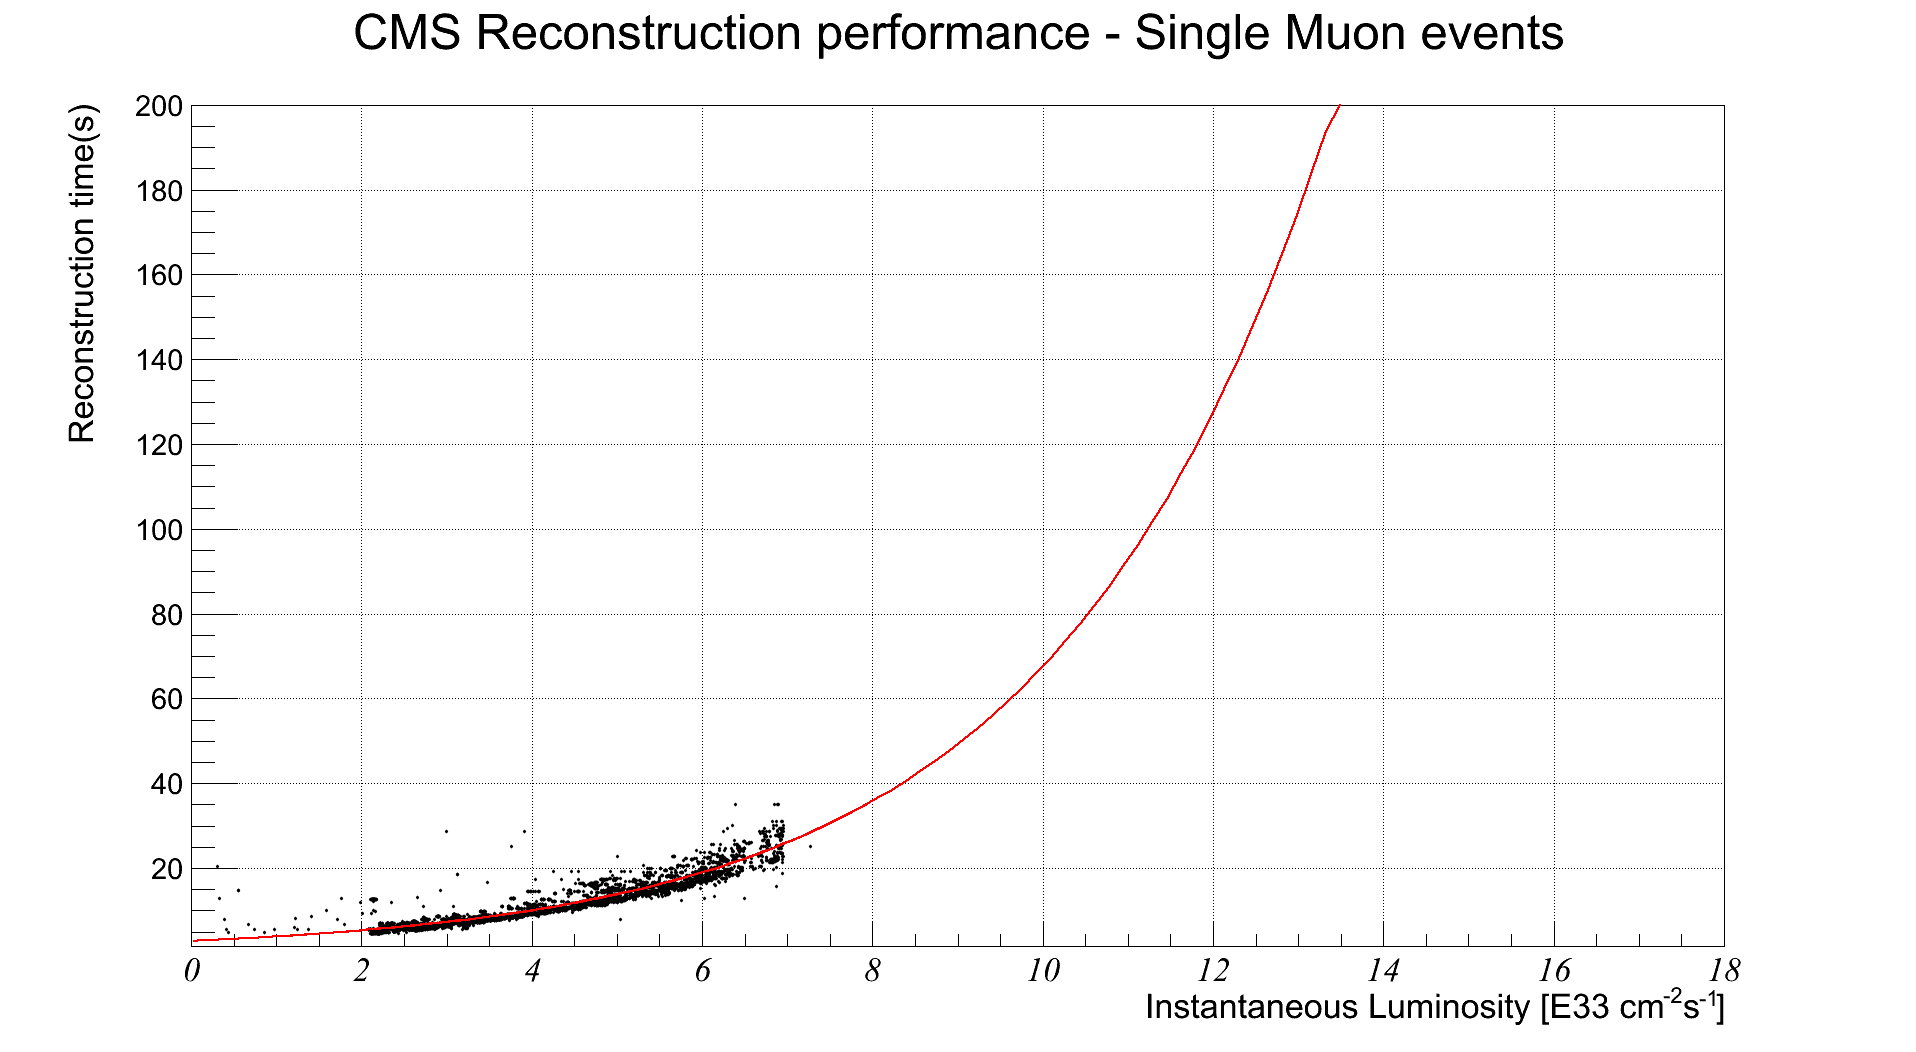
\includegraphics[width=100mm]{lumitpeSingleMu-fitted2.png}
    \caption{\label{lumitpeSingleMu} Event processing time versus
      instantaneous luminosity.}
\end{figure}

\bibliographystyle{h-elsevier}
\bibliography{collaborative_proposal}{}
%\bibliography{auto_generated}

\end{document}

% LocalWords:  Exascale LHC Ko Rappoccio Lukasz Zialek Ziarek EIC PIs
% LocalWords:  Collider exascale transformative CMS multicore VMs bla
% LocalWords:  luminosities HEP HTC HPC hadrons hadronic fastjet NN
% LocalWords:  Ref kNN Refs knn gpu factorized
